\documentclass[a4paper, listof=totoc]{scrreport}
\usepackage{attitude_control}

\newglossaryentry{sy:dcm}{
    name = \ensuremath{\mat{C}},
    description = {\gls{ac:dcm}},
    sort = C,
    type = symbols,
}

\newglossaryentry{sy:c1}{
    name = \ensuremath{\mat{C_1}},
    description = {Single axis rotation matrix for roll},
    sort = C1,
    type = symbols,
}

\newglossaryentry{sy:c2}{
    name = \ensuremath{\mat{C_2}},
    description = {Single axis rotation matrix for pitch},
    sort = C2,
    type = symbols,
}

\newglossaryentry{sy:c3}{
    name = \ensuremath{\mat{C_3}},
    description = {Single axis rotation matrix for yaw},
    sort = C3,
    type = symbols,
}

\newglossaryentry{sy:roll}{
    name = \ensuremath{\theta_1},
    description = {Roll angle},
    sort = theta1,
    type = symbols,
}

\newglossaryentry{sy:pitch}{
    name = \ensuremath{\theta_2},
    description = {Pitch angle},
    sort = theta2,
    type = symbols,
}

\newglossaryentry{sy:yaw}{
    name = \ensuremath{\theta_3},
    description = {Pitch angle},
    sort = theta3,
    type = symbols,
}


\subject{Attitude Dynamics and Control (AE4313)}
\title{Nonlinear Spacecraft Attitude Control System Design}
\subtitle{Practical Exercise Project Assignment 2}
\author{Lars Blümler\\6149065}
\publishers{\includegraphics{tu_delft_logo.pdf}}


\begin{document}
% front matter
\maketitle
\pagenumbering{roman}
\tableofcontents
\listoffigures
%\begingroup
    %\let\clearpage\relax
    %\listoftables
%\endgroup
\clearpage


% main matter
\pagenumbering{arabic}
\chapter{Methodology}
\section{Coordinate Systems}
\begin{figure}[!htb]
    \centering
    \captionbox{Inertial frame}{

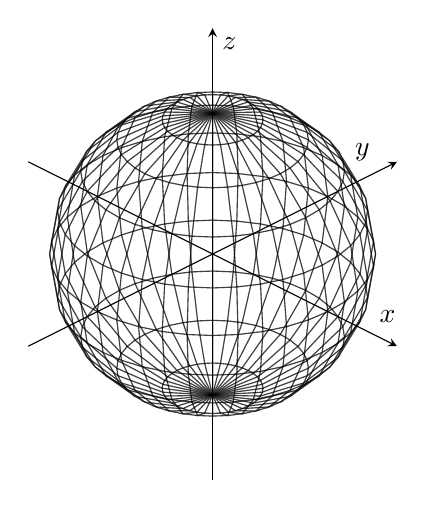
\begin{tikzpicture}
    \begin{axis}[
        height=12cm,
        axis equal,
        axis lines = center, 
        xlabel = {$x$},
        ylabel = {$y$},
        zlabel = {$z$},
        ticks=none,
        enlargelimits=0.3,
        view/h=45,
        scale uniformly strategy=units only,
    ]
    \addplot3[%
        opacity = 0.5,
        mesh,
        draw = black,
        z buffer = sort,
        samples = 21,
        variable = \u,
        variable y = \v,
        domain = 0:180,
        y domain = 0:360,
    ]
    ({cos(u)*sin(v)}, {sin(u)*sin(v)}, {cos(v)});
    \end{axis}
\end{tikzpicture}

   }
   \captionbox{LVLH frame}{

\begin{tikzpicture}
    \begin{axis}[
        height=12cm,
        axis equal,
        axis lines = center, 
        xlabel = {$x$},
        ylabel = {$y$},
        zlabel = {$z$},
        ticks=none,
        %enlargelimits=0.3,
        view/h=135,
        view/v=135,
        scale uniformly strategy=units only,
    ]
    \addplot3[%
        opacity = 0.5,
        mesh,
        draw = black,
        samples = 21,
        variable = \u,
        domain = 60:120,
    ]
    ({cos(u)}, {sin(u)-1}, 0);
    \addplot3[opacity = 0] (0, 1, 0);
    \addplot3[opacity = 0] (1, 0, 0);
    \addplot3[opacity = 0] (0, 0, 1);
    \end{axis}
\end{tikzpicture}

   }
\end{figure}
Three coordinate systems are used in this report: the inertial frame, the \gls{lvlh} frame, and the body frame.
The inertial frame is supposed to be unaccelerated fixed to the center of Earth.
The \gls{lvlh} frame is centered at the spacecraft and rotates with the spacecraft's orbit.
The body frame is the reference frame used for by the spacecraft itself and thus rotates with the spacecraft's attitude.
The attitude is then the transformation from the \gls{lvlh} frame to the body frame.



\section{Attitude Representation}
\subsection{\texorpdfstring{\acrlong{ac:dcm}}{Direction Cosine Matrix}}
The \glsfull{sy:dcm} is a matrix that describes the linear transformation between two coordinate frames.
In three dimension, $\gls{sy:dcm} \in \mathbb{R}^{3 \times 3}$ and the definition is given by \cref{eqt:dcm}.
\begin{equation} \label{eqt:dcm}
    \gls{sy:dcm} = \begin{bmatrix}
        \gls{sy:dcm}_{11} & \gls{sy:dcm}_{12} & \gls{sy:dcm}_{13} \\
        \gls{sy:dcm}_{21} & \gls{sy:dcm}_{22} & \gls{sy:dcm}_{23} \\
        \gls{sy:dcm}_{31} & \gls{sy:dcm}_{32} & \gls{sy:dcm}_{33}
    \end{bmatrix}
\end{equation}

A transformation matrix $\gls{sy:dcm}^{B/A}$ from frame $A$ to frame $B$ is constructed from the basis vectors of frame $A$ ($\gls{sy:a}_1$, $\gls{sy:a}_2$, $\gls{sy:a}_3$) as expressed in frame $B$ ($\gls{sy:b}_1$, $\gls{sy:b}_2$, $\gls{sy:b}_3$).
In the case of both bases consisting of unit vectors, the \gls{ac:dcm} elements become equal to the cosine of the angle between each pair of basis vectors (see \cref{eqt:dcm_basis}), hence the name cosine matrix.
\begin{equation} \label{eqt:dcm_basis}
    \gls{sy:dcm}^{B/A} = \begin{bmatrix}
        \gls{sy:b}_1 \cdot \gls{sy:a}_1 & \gls{sy:b}_1 \cdot \gls{sy:a}_2 & \gls{sy:b}_1 \cdot \gls{sy:a}_3 \\
        \gls{sy:b}_2 \cdot \gls{sy:a}_1 & \gls{sy:b}_2 \cdot \gls{sy:a}_2 & \gls{sy:b}_2 \cdot \gls{sy:a}_3 \\
        \gls{sy:b}_3 \cdot \gls{sy:a}_1 & \gls{sy:b}_3 \cdot \gls{sy:a}_2 & \gls{sy:b}_3 \cdot \gls{sy:a}_3
    \end{bmatrix}
    =
    \begin{bmatrix}
        \cos \theta_{11} & \cos \theta_{12} & \cos \theta_{13} \\
        \cos \theta_{21} & \cos \theta_{22} & \cos \theta_{23} \\
        \cos \theta_{31} & \cos \theta_{32} & \cos \theta_{33}
    \end{bmatrix}
\end{equation}


\subsubsection*{Single Axis Rotations}
For any single axis rotation about axis $i$ with angle $\theta_i$, the rotation axis remains unchanged leaving $\gls{sy:a}_i = \gls{sy:b}_i$.
The resulting \glspl{ac:dcm} are given by \cref{eqt:c1,eqt:c2,eqt:c3}.

\parbox{.49\textwidth}{
\begin{equation} \label{eqt:c1}
    \gls{sy:c1}(\gls{sy:roll}) = \begin{bmatrix}
        1 & 0 & 0 \\
        0 & \cos(\gls{sy:roll}) & \sin(\gls{sy:roll}) \\
        0 & -\sin(\gls{sy:roll}) & \cos(\gls{sy:roll})
    \end{bmatrix}
\end{equation}
}
\parbox{.49\textwidth}{
\begin{equation} \label{eqt:c2}
    \gls{sy:c2}(\gls{sy:pitch}) = \begin{bmatrix}
        \cos(\gls{sy:pitch}) & 0 & -\sin(\gls{sy:pitch}) \\
        0 & 1 & 0 \\
        \sin(\gls{sy:pitch}) & 0 & \cos(\gls{sy:pitch})
    \end{bmatrix}
\end{equation}
}
\begin{equation} \label{eqt:c3}
    \gls{sy:c3}(\gls{sy:yaw}) = \begin{bmatrix}
        \cos(\gls{sy:yaw}) & \sin(\gls{sy:yaw}) & 0 \\
        -\sin(\gls{sy:yaw}) & \cos(\gls{sy:yaw}) & 0 \\
        0 & 0 & 1
    \end{bmatrix}
\end{equation}


\subsection{Euler Angles}
Euler angles are a set of three angles that represent an orientation, rotation or attitude as three successive, single axis rotations.
The rotations can be performed about any axis in any order, so long as no two rotations are about the same axis.
For each successive rotation is applied to the intermediate frame, resulting from the previous rotation.
This leads to two intermediate frames being created $A \overset{i}{\rightarrow} A' \overset{j \neq i}{\rightarrow} A'' \overset{k \neq j}{\rightarrow} B$.

Defining a triplet with rotation order $3 \rightarrow 2 \rightarrow 1$, any attitude can then be represented by a triplet of roll, pitch and yaw Euler angles (see \cref{eqt:ypr_attitude}).
\begin{equation} \label{eqt:ypr_attitude}
    \gls{sy:ypr} = \begin{bmatrix}
        \gls{sy:roll} \\
        \gls{sy:pitch} \\
        \gls{sy:yaw}
    \end{bmatrix}
\end{equation}


\subsubsection*{Euler Angles to DCM}
Using a $3 \rightarrow 2 \rightarrow 1$ rotation sequence using the \glsfull{sy:yaw}, \glsfull{sy:pitch} and \glsfull{sy:roll}, the resulting \gls{ac:dcm} is given by \cref{eqt:dcm_euler}.
\begin{gather} \label{eqt:dcm_euler}
    \gls{sy:dcm} = \gls{sy:c1}(\gls{sy:roll}) \, \gls{sy:c2}(\gls{sy:pitch}) \, \gls{sy:c3}(\gls{sy:yaw}) \\
    = \\ \begin{bmatrix}
        \cos \gls{sy:pitch} \cos \gls{sy:yaw}
        &
        \cos \gls{sy:pitch} \sin \gls{sy:yaw}
        & -\sin \gls{sy:pitch}
        \\
        \sin \gls{sy:roll} \sin \gls{sy:pitch} \cos \gls{sy:yaw} - \cos \gls{sy:roll} \sin \gls{sy:yaw}
        &
        \cos \gls{sy:roll} \cos \gls{sy:yaw} + \sin \gls{sy:roll} \sin \gls{sy:pitch} \sin \gls{sy:yaw}
        &
        \sin \gls{sy:roll} \cos \gls{sy:pitch}
        \\
        \sin \gls{sy:roll} \sin \gls{sy:yaw} + \cos \gls{sy:roll} \sin{\gls{sy:pitch}} \cos \gls{sy:yaw}
        &
        \cos{\gls{sy:roll}} \sin{\gls{sy:pitch}} \sin \gls{sy:yaw} - \sin \gls{sy:roll} \cos \gls{sy:yaw} 
        &
        \cos{\gls{sy:roll}} \cos \gls{sy:pitch}
    \end{bmatrix}
\end{gather}


\subsection{Eigenaxis Rotations}
For every rotation between two frames, there exists a unique axis of rotation, for which the coordinates are equal in both frames of reference (see \cref{eq:eigenaxis_definition}).
\begin{equation} \label{eq:eigenaxis_definition}
    \gls{sy:e} = e_1 \gls{sy:b}_1 + e_2 \gls{sy:b}_2 + e_3 \gls{sy:b}_3 = e_1 \gls{sy:a}_1 + e_2 \gls{sy:a}_2 + e_3 \gls{sy:a}_3
\end{equation}

Any rotation can then be described using the eigenaxis of the rotation and the angle of rotation about that axis.
The \gls{ac:dcm} for a rotation about the eigenaxis $\gls{sy:e}$ with angle $\gls{sy:theta}$ is given by \cref{eqt:eigenaxis_dcm}.
\begin{equation} \label{eqt:eigenaxis_dcm}
    \gls{sy:dcm}(\gls{sy:e}, \gls{sy:theta}) = \begin{bmatrix}
        \cos{\gls{sy:theta}} + e_1^2 (1 - \cos{\gls{sy:theta}}) 
        &
        e_1 e_2 (1 - \cos{\gls{sy:theta}}) + e_3 \sin{\gls{sy:theta}}
        &
        e_1 e_3 (1 - \cos{\gls{sy:theta}}) - e_2 \sin{\gls{sy:theta}}
        \\
        e_2 e_1 (1 - \cos{\gls{sy:theta}}) - e_3 \sin{\gls{sy:theta}}
        &
        \cos{\gls{sy:theta}} + e_2^2 (1 - \cos{\gls{sy:theta}})
        &
        e_2 e_3 (1 - \cos{\gls{sy:theta}}) + e_1 \sin{\gls{sy:theta}}
        \\
        e_3 e_1 (1 - \cos{\gls{sy:theta}}) + e_2 \sin{\gls{sy:theta}}
        &
        e_3 e_2 (1 - \cos{\gls{sy:theta}}) - e_1 \sin{\gls{sy:theta}}
        &
        \cos{\gls{sy:theta}} + e_3^2 (1 - \cos{\gls{sy:theta}})
    \end{bmatrix}
\end{equation}

For subsequent rotations, the equivalent Eigenaxis rotation can be computed by solving $\gls{sy:dcm}(\gls{sy:e}, \gls{sy:theta}) = \gls{sy:dcm}(\gls{sy:e}_2, \gls{sy:theta}_2) \gls{sy:dcm}(\gls{sy:e}_1, \gls{sy:theta}_1)$.
This results in the equivalent eigenaxis rotation given in \cref{eqt:eigenaxis_product}.
\begin{equation} \label{eqt:eigenaxis_product}
    \gls{sy:e} \sin{\frac{\gls{sy:theta}}{2}}
    =
    \gls{sy:e}_1 \sin{\frac{\gls{sy:theta}_1}{2}} \cos{\frac{\gls{sy:theta}_2}{2}}
    + \gls{sy:e}_2 \sin{\frac{\gls{sy:theta}_2}{2}} \cos{\frac{\gls{sy:theta}_1}{2}}
    + (\gls{sy:e}_1 \times \gls{sy:e}_2) \sin{\frac{\gls{sy:theta}_1}{2}} \sin{\frac{\gls{sy:theta}_2}{2}}
\end{equation}


\subsection{Quaternions}
We define a quaternion \gls{sy:q} as a four-dimensional vector with one scalar and three vector components, as shown in \cref{eqt:quaternion}.
\begin{equation} \label{eqt:quaternion}
    \gls{sy:q} = \begin{bmatrix}
        q_1 \\
        q_2 \\
        q_3 \\
        q_4
    \end{bmatrix}
    =
    \begin{bmatrix}
        e_1 \, \sin(\frac{\theta}{2}) \\
        e_2 \, \sin(\frac{\theta}{2}) \\
        e_3 \, \sin(\frac{\theta}{2}) \\
        \cos(\frac{\theta}{2})
    \end{bmatrix}
\end{equation}
Where \gls{sy:e} is the unit vector of the eigenaxis of the rotation and \gls{sy:theta} is the rotation angle.
With $|\gls{sy:e}_i| = 1$, the components are not independent of each other and underlie the constraint of a unit norm $q_1^2 + q_2^2 + q_3^2 + q_4^2 = 1$.

This definition allows for a representation of subsequent rotations as given in \cref{eqt:quaternion_product} without the use of trigonometric functions.
\begin{equation} \label{eqt:quaternion_product}
    \gls{sy:q}^B = \begin{bmatrix}
         q_4^{B/A} &  q_3^{B/A} & -q_2^{B/A} & q_1^{B/A} \\
        -q_3^{B/A} &  q_4^{B/A} &  q_1^{B/A} & q_2^{B/A} \\
         q_2^{B/A} & -q_1^{B/A} &  q_4^{B/A} & q_3^{B/A} \\
        -q_1^{B/A} & -q_2^{B/A} & -q_3^{B/A} & q_4^{B/A} 
    \end{bmatrix}    
    \,
    \begin{bmatrix}
        q_1^A \\
        q_2^A \\
        q_3^A \\
        q_4^A
    \end{bmatrix}
\end{equation}


\subsubsection*{Quaternions to DCM}
Using this definition of quaternions, the corresponding \gls{sy:dcm} for a given quaternion can be expressed as shown in \cref{eqt:quaternion_to_dcm}. 
\begin{equation} \label{eqt:quaternion_to_dcm}
    \gls{sy:dcm} = \begin{bmatrix}
        1 - 2(q_2^2 + q_3^2) & 2(q_1 q_2 + q_3 q_4) & 2(q_1 q_3 - q_2 q_4) \\
        2(q_1 q_2 + q_3 q_4) & 1 - 2(q_1^2 + q_3^2) & 2(q_2 q_3 + q_1 q_4) \\
        2(q_1 q_3 + q_2 q_4) & 2(q_2 q_3 - q_1 q_4) & 1 - 2(q_1^2 + q_2^2)
    \end{bmatrix}
\end{equation}

Inversely, the quaternion can be calculated from the \glsdesc{sy:dcm} as shown in \cref{eqt:dcm_to_quaternion}.
\begin{equation} \label{eqt:dcm_to_quaternion}
    \gls{sy:q} = \frac{1}{4 q_4} \begin{bmatrix}
        \gls{sy:dcm}_{23} - \gls{sy:dcm}_{32} \\
        \gls{sy:dcm}_{31} - \gls{sy:dcm}_{13} \\
        \gls{sy:dcm}_{12} - \gls{sy:dcm}_{21}
    \end{bmatrix}
\end{equation}

This reveals a singularity for $q_4 = 0$, which occurs for rotations about the eigenaxis of $\pi$ radians, for which the quaternion becomes undefined.


\subsubsection*{Single Axis Rotations}
Using the definition of single axis rotation in \gls{ac:dcm} representation (\cref{eqt:c1,eqt:c2,eqt:c3}), together with the relationship between \gls{sy:dcm} and quaternions (\cref{eqt:quaternion_to_dcm}), we can derive the single axis rotation matrices in quaternion representation as shown in \cref{eqt:quaternion_c1,eqt:quaternion_c2,eqt:quaternion_c3}.

\parbox{.32\textwidth}{
\begin{equation} \label{eqt:quaternion_c1}
    \gls{sy:q}^{C_1} = \begin{bmatrix}
        \sin \frac{\gls{sy:roll}}{2} \\
        0 \\
        0 \\
        \cos \frac{\gls{sy:roll}}{2}
    \end{bmatrix}
\end{equation}
}
\parbox{.32\textwidth}{
\begin{equation} \label{eqt:quaternion_c2}
    \gls{sy:q}^{C_2} = \begin{bmatrix}
        0 \\
        \sin \frac{\gls{sy:pitch}}{2} \\
        0 \\
        \cos \frac{\gls{sy:pitch}}{2}
    \end{bmatrix}
\end{equation}
}
\parbox{.32\textwidth}{
\begin{equation} \label{eqt:quaternion_c3}
    \gls{sy:q}^{C_3} = \begin{bmatrix}
        0 \\
        0 \\
        \sin \frac{\gls{sy:yaw}}{2} \\
        \cos \frac{\gls{sy:yaw}}{2}
    \end{bmatrix}
\end{equation}
}


\subsubsection*{Euler Angles to Quaternions}
Using the yaw $\rightarrow$ pitch $\rightarrow$ roll rotation sequence, the quaternion can be expressed as a function of the Euler angles using the single axis rotation quaternions (\cref{eqt:quaternion_c1,eqt:quaternion_c2,eqt:quaternion_c3}).
The resulting quaternion as shown in \cref{eqt:ypr_to_quaternion}.
\begin{equation} \label{eqt:ypr_to_quaternion}
    \gls{sy:q} = \begin{bmatrix}
        \sin \frac{\gls{sy:roll}}{2} \cos \frac{\gls{sy:pitch}}{2} \cos \frac{\gls{sy:yaw}}{2} 
        - \cos \frac{\gls{sy:roll}}{2} \sin \frac{\gls{sy:pitch}}{2} \sin \frac{\gls{sy:yaw}}{2}
        \\
        \cos \frac{\gls{sy:roll}}{2} \sin \frac{\gls{sy:pitch}}{2} \cos \frac{\gls{sy:yaw}}{2} 
        + \sin \frac{\gls{sy:roll}}{2} \cos \frac{\gls{sy:pitch}}{2} \sin \frac{\gls{sy:yaw}}{2}
        \\
        \cos \frac{\gls{sy:roll}}{2} \cos \frac{\gls{sy:pitch}}{2} \sin \frac{\gls{sy:yaw}}{2}
        - \sin \frac{\gls{sy:roll}}{2} \sin \frac{\gls{sy:pitch}}{2} \cos \frac{\gls{sy:yaw}}{2}
        \\
        \cos \frac{\gls{sy:roll}}{2} \cos \frac{\gls{sy:pitch}}{2} \cos \frac{\gls{sy:yaw}}{2}
        + \sin \frac{\gls{sy:roll}}{2} \sin \frac{\gls{sy:pitch}}{2} \sin \frac{\gls{sy:yaw}}{2}
    \end{bmatrix}
\end{equation}
\section{Kinematics}
\subsection{Orbit Kinematics}
Treated in this exercise is a spacecraft in a circular orbit of \glsdesc{sy:h} \qty{700}{\km} around Earth.
The orbital frequency or \glsdesc{sy:mean_motion} is calculated using \cref{eqt:mean_motion}.
\begin{equation} \label{eqt:mean_motion}
    \gls{sy:mean_motion} = \sqrt{\frac{\gls{sy:mu_earth}}{\gls{sy:r}^3}} = \sqrt{\frac{\gls{sy:mu_earth}}{(\gls{sy:r}_E + h)^3}}
\end{equation}

Using $\gls{sy:mu_earth} = \qty{3.98600442e14}{\meter^3\per\second^2}$ and $\gls{sy:r}_E = \qty{6.378137e6}{\m}$, the mean motion is calculated to be $\gls{sy:mean_motion} = \qty{1.060206e-3}{\per\second}$.

\section{Dynamics}
The torque acting on a rigid body can be expressed as
\begin{equation} \label{eqt:torque}
    \vec{T} = \gls{sy:j} \gls{sy:omega_dot} + \gls{sy:omega} \times \gls{sy:j} \gls{sy:omega}
\end{equation}
The resulting angular acceleration from a given torque can thus be expressed as
\begin{equation} \label{eqt:angular_acceleration}
    \gls{sy:omega_dot} = \gls{sy:j}^{-1} \left( \vec{T} - \gls{sy:omega} \times \gls{sy:j} \gls{sy:omega} \right)
\end{equation}
When splitting the total torque into control and disturbance torques $\vec{T} = \gls{sy:t_c} + \gls{sy:t_d}$, the equation can be rewritten as
\begin{equation} \label{eqt:torque_split}
    \gls{sy:omega_dot} = \gls{sy:j}^{-1} \left( \gls{sy:t_d} - \gls{sy:omega} \times \gls{sy:j} \gls{sy:omega} \right)
    + \gls{sy:j}^{-1} \gls{sy:t_c}
\end{equation}



\section{Controller Design}
\subsection{Linearization}
\subsection{\texorpdfstring{\acrlong{pd}}{Proportional Differential} Controller}
\subsection{\texorpdfstring{\acrlong{ndi}}{Nonlinear Dynamic Inversion}}
\subsection{\texorpdfstring{\acrlong{tss}}{Time Scale Separation}}
\subsection{\texorpdfstring{\acrlong{indi}}{Incremental Dynamic Inversion}}



\chapter{Results}

\begin{figure}
    \centering
    \captionbox{Attitudes of spacecraft using a linear state feedback controller.\label{fig:attitudes_state_feedback_controller_ypr}}{
    \includegraphics[width=.95\textwidth]{attitudes_StateFeedbackController_YawPitchRoll}
    }
    \captionbox{Attitude errors of spacecraft using a linear state feedback controller.\label{fig:attitude_errors_state_feedback_controller_ypr}}{
    \includegraphics[width=.95\textwidth]{attitude_errors_StateFeedbackController_YawPitchRoll}
    }
    \captionbox{Control torques of spacecraft using a linear state feedback controller.\label{fig:control_torques_state_feedback_controller_ypr}}{
    \includegraphics[width=.95\textwidth]{control_torques_StateFeedbackController_YawPitchRoll}
    }
\end{figure}



\chapter{Discussion}
The NDI controller shows remarkable performance in the simulation.
This is due to the fact that the NDI controller relies on its full model for the inversion, which in this case is the same as is being used for the simulation, thus achieving a perfect inversion.
Normally, NDI would be limited by uncertainties in i.e. the attitude measurements, inertia matrix, and disturbance torques.

This heavy model reliance is also clear when observing the performance using quaternions.
A model error here leads to a divergence of the controller after the second attitude maneuver.
While the error was unfortunately unable to be fixed due to the complex model, this highlights the weakness of a heavy model reliance.

The state feedback controller on the other hand performs according to expectations well around the equilibrium point.
It starts oscillating much heavier using off nadir maneuvers, which is expected as the controller is not designed for this.
An alternative would be to use multiple controllers, one lineaerized around each attitude and switching between them.

The TSS and INDI controllers both show a similar performance, with the INDI controller performing better in steady state divergence.
Both controllers good performance in all attitude ranges show the advantages of the reduced model reliance while maintaining a good performance.

Quaternion based control suffered from a steady state divergence in all controllers.
This is most likely due to a wrong computation of the error quaternion as steady state convergence is seen in every case.
This indicates that the error quaternion does indeed converge to zero, thus the steady state divergence is not due to a wrong control input, but rather a wrong error computation.



% back matter
\printglossary[type=\acronymtype]
\begingroup
    \let\clearpage\relax
    \printglossary[type=symbols, style=long3col]
\endgroup
\printbibliography

\end{document}
